\documentclass[]{article}
\usepackage[a4paper, total={6in, 8in}]{geometry}
\usepackage[english]{babel}	
\usepackage[utf8]{inputenc} % Umlaute
\usepackage{amssymb}
\usepackage{amsmath} 
\usepackage{fancyhdr}
\usepackage{fancyvrb} % Für regex Umgebung
\usepackage{multicol} % Mehrere Spalten
\usepackage{graphicx} % bilder
\usepackage[table]{xcolor}
\usepackage{hyperref}
\pagestyle{fancy} 
\fancyhf{} %clears the header and footer
\rhead{Professor Robert Feldmann (lectures) \\ Dr. Darren Reed (exercise classes) \\ Dimakopoulos Vasileios (TA) \\ Elia Cenci (TA)}
\lhead{Universität Zürich \\ Institute for Computational Science \\ Spring Semester 2021 \\ ESC403}
\fancyfoot[C]{\thepage}


\title{\textbf{INTRODUCTION TO DATA SCIENCE FINAL EXAM 2021}}
\author{Solutions from David Linder}

\begin{document}
\maketitle
\thispagestyle{fancy}
\section{Time Series}
\subsection{}
To be considered stationary a time series should have the following properties:
\begin{itemize}
	\item The mean $E[X_t]$ is the same for all times $t$
	\item The variance $Var[X_t]$ is the same for all times $t$
	\item The covariance between $X_t$ and $X_{t-1}$ is the same for all $t, n$
\end{itemize}
That means we want
\begin{itemize}
	\item no obvious trends
	\item constant variance with time
	\item constant autocorrelation structure over time
	\item no periodic fluctuations (no seasonality)
\end{itemize}
I found some examples \href{https://otexts.com/fpp2/stationarity.html}{here}: In figure \ref{fig:time_series} we see that most of the series are non-stationary except series (b) and (g). In series (g) there are cycles but they are not periodic. 
\begin{figure}
	\centering
	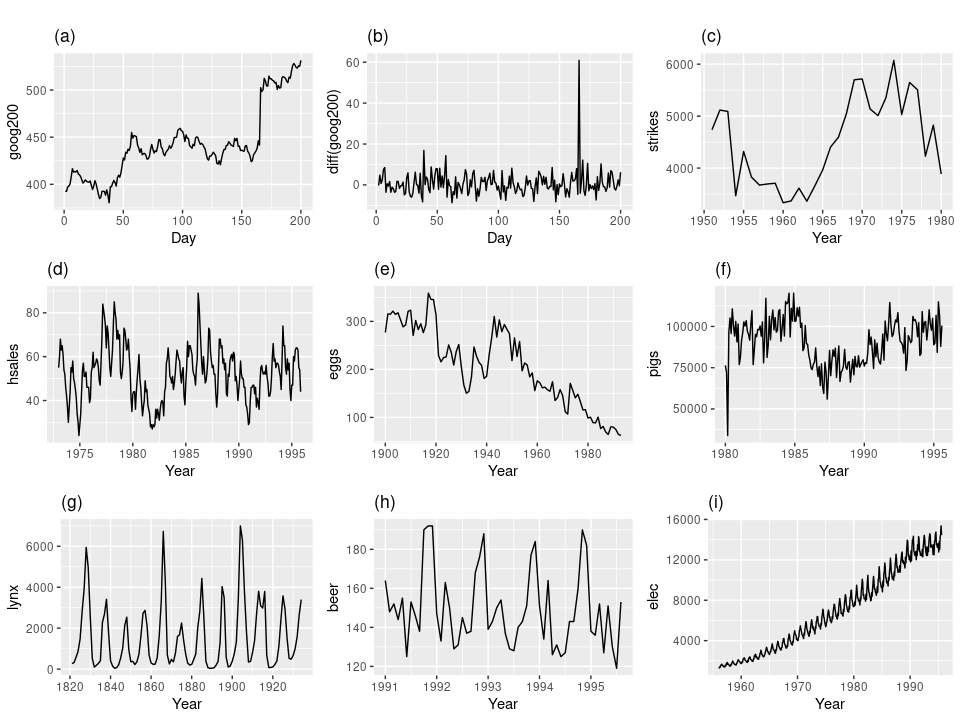
\includegraphics[width=1\textwidth]{images/time_series.png}
		\caption{(a) Google stock price for 200 consecutive days; (b) Daily change in the Google stock price for 200 consecutive days; (c) Annual number of strikes in the US; (d) Monthly sales of new one-family houses sold in the US; (e) Annual price of a dozen eggs in the US (constant dollars); (f) Monthly total of pigs slaughtered in Victoria, Australia; (g) Annual total of lynx trapped in the McKenzie River district of north-west Canada; (h) Monthly Australian beer production; (i) Monthly Australian electricity production.}
		\label{fig:time_series}
\end{figure}

\subsection{}
\subsection{}
\section{Image classification}
\subsection{}
\subsection{}
\subsection{}
\subsection{}
\subsection{Bonus Question}
\end{document}